\documentclass[a4paper, twoside]{report}

%% Language and font encodings
\usepackage[english]{babel}
\usepackage[superscript,biblabel]{cite} %% Small superscript references
\usepackage[utf8x]{inputenc}
\usepackage[T1]{fontenc}

%% Sets page size and margins
\usepackage[a4paper,top=3cm,bottom=2cm,left=3cm,right=3cm,marginparwidth=1.75cm]{geometry}

%% Useful packages
\usepackage{amsmath}
\usepackage{amssymb}
\usepackage{graphicx}
\usepackage{caption}
\usepackage{subcaption}
\usepackage[colorinlistoftodos]{todonotes}
\usepackage[colorlinks=true, allcolors=blue]{hyperref}

%% Technical drawing package
\usepackage{tikz}
\usetikzlibrary{arrows,chains,matrix,positioning,scopes,decorations.pathmorphing,math}

%% Math commands for formatting
\newcommand{\matr}[1]{\mathbf{#1}}
\DeclareMathOperator{\diag}{diag}

\title{Emulating the Quantum Valley Hall Effect in Topologically Perturbed Model Systems}
\author{Bernard Ting}

\begin{document}
\input{title/title.tex}

\begin{abstract}
We investigate how the topological pertubation of an elastic mass-spring system
leads to the formation of bandgaps which behave similarly to the quantum
valley-Hall effect. We first introduce the theory of dispersion curves and plot
them for simple models. We then break the symmetry by introducing masses of
different weights and observe induces a bandgap. The resulting structures
composed of two media with different topological invariants have non-trivial
bandgaps which support edge waves at the interface. We analyse the dispersion
relations on the unit cell and finite strip to find special frequencies or
modes which are present in the band gap. Numerical scattering simulations are
then run with these frequencies induced to the lattice to confirm our analysis.
This work proposes several different ways of topologically perturbing lattices
as well as seek to show that this simple model is able to emulate the
behaviours and effects seen in more complex systems.
\end{abstract}

\renewcommand{\abstractname}{Acknowledgements}
\begin{abstract}
I would like to extend my greatest thanks to my supervisor, Prof. Richard
Craster, for his advice and guidance on all matters relating to the project. I
would also like to thank Dr. Christopher Ford for being my second marker and
providing timely feedback regarding my project.
\end{abstract}

\tableofcontents
%% \listoffigures
%% \listoftables

\chapter{Introduction}
The study of metamaterials has the potential to solve many modern engineering
problems.

\section{Objectives}
\begin{itemize}
\item Perturb structures of semi-infinite lattices to open up band gaps
\item Simulate scattering to confirm dissipation of energy
\end{itemize}

\chapter{Background}
Waves exhibit many characteristics when travelling through different mediums. 

\section{Dispersion relation}
A dispersion relation relates the wavenumber of a wave to its frequency. We
will see that this relation is of utmost importance when discussing lattices as
only waves of certain frequencies are transmitted by the lattice.

\subsection{1D lattice}
Let us start our discussion with the most basic one-dimensional case. In this
case, we have masses of equal mass, $m$ spread out evenly across one dimension.
All neighbouring masses are connected by an elastic force which scales
proportionally with distance, i.e. $F = kx$ for some $k$.

% TODO: Add discussion about transverse waves into appendix?
\textit{Note}: It is very useful to think of this system as a mass-spring
system. For simplicity, we will be considering longitudinal waves, however the
same analysis can be done for transverse waves as we show in the appendix.

With this one-dimensional case set up, we now want to find out what forms of
waves it allows to propagate. We do this by examining the elementary unit of
the lattice which can be repeated by translation to form the full lattice.

So let us consider three masses side-by-side in our lattice, $M_{n-1}$, $M_n$
and $M_{n+1}$ which are $y_{n-1}$, $y_n$ and $y_{n+1}$ displacement away from
their equilibrium positions. By focusing on the centre mass and considering
only nearest neighbour interactions, by Hooke's Law, we have that the force on
$M_n$

\begin{align}
  F_{n}=\sum F=k\left(y_{n-1}+y_{n+1}-2y_{n}\right) \label{eq:HL}
\end{align}

At the same time, we have by Newton's 2nd Law that

\begin{align}
  F_{n}=m\frac{d^{2}}{dt^{2}}y_{n}
\end{align}

Taking $y_n$ to be the general wave solution

\begin{align}
  &y_{n}=\hat{y}_{n}e^{-i\Omega t} \\
  \Rightarrow &\frac{d^{2}}{dt^{2}}y_{n}=-\Omega^{2}y_{n} \\
  \Rightarrow &F_{n}=-m\Omega^{2}y_{n}a \label{eq:N2L}
\end{align}

where $\Omega$ is the frequency of the wave and $\hat{y}_{n}$ is the complex
amplitude.

Therefore, we have by \eqref{eq:HL} and \eqref{eq:N2L} that

\begin{align}
  &-m\Omega^{2}y_{n}=k\left(y_{n-1}+y_{n+1}-2y_{n}\right) \\
  \Rightarrow &\left(-\frac{m}{k}\Omega^{2}+2\right)y_{n}-y_{n-1}-y_{n+1}=0
    \label{eq:HLN2L}
\end{align}

Now since we have that $M_{n-1}$ and $M_{n+1}$ are equidistant from $M_{n}$ at
equilibrium, we can describe the phase shift in the wave solution as

\begin{align}
  y_{n-1}=e^{-i\kappa}y_n,\ \ y_{n+1}=e^{i\kappa}y_n
\end{align}

Hence, from \eqref{eq:HLN2L}, we see that

\begin{align}
  &\left(-\frac{m}{k}\Omega^{2}+2-e^{-i\kappa}-e^{i\kappa}\right)y_{n}=0 \\
  \Rightarrow &\cos\left(\kappa\right)=\frac{2m}{k}\Omega^{2}+4
\end{align}

\subsection{1D lattice with two masses}

\subsection{2D square lattice}

\subsection{2D square lattice with two masses}

\chapter{Dispersion relation}
\label{disperrel}
A dispersion relation relates the wavenumber of a wave to its frequency. We
will see that this relation is of utmost importance when discussing periodic
lattices as only waves of certain frequencies are transmitted by the lattice.

\section{1d lattice}
\begin{center}
  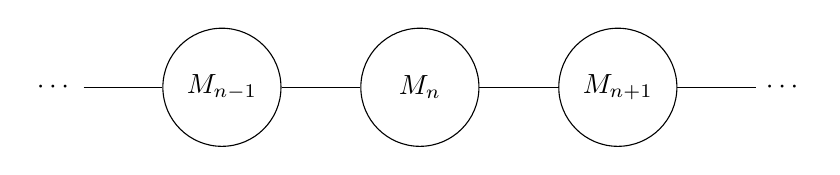
\begin{tikzpicture}
  {[start chain,every on chain/.style=join,every join/.style=-,
    state/.style={circle,draw,minimum size=1.5cm}]
     \node[on chain] (A) {$\cdots$};
     \node[on chain,state] (B) {$M_{n-1}$};
     \node[on chain,state] (C) {$M_n$};
     \node[on chain,state] (D) {$M_{n+1}$};
     \node[on chain] (E) {$\cdots$};
  }
  \end{tikzpicture}
\end{center}
Let us start our discussion with the most basic one-dimensional case. In this
case, we have masses of equal mass, $m$ spread out evenly across one dimension.
All neighbouring masses are connected by an elastic force which scales
proportionally with distance, i.e. $F = kx$ for some $k$.

% TODO: Add discussion about transverse waves into appendix?
\textit{Note}: It is very useful to think of this system as a mass-spring
system. For simplicity, we will be considering longitudinal waves, however the
same analysis can be done for transverse waves as we show in the appendix.

With this one-dimensional case set up, we now want to find out what forms of
waves it allows to propagate. We do this by considering only nearest neighbour
interactions and examining the elementary unit of the lattice which can be
repeated by translation to form the full lattice.

So let us consider three masses side-by-side in our lattice, $M_{n-1}$, $M_n$
and $M_{n+1}$ which are $y_{n-1}$, $y_n$ and $y_{n+1}$ displacement away from
their equilibrium positions. By focusing on the centre mass and considering
only nearest neighbour interactions, by Hooke's Law, we have that the force on
$M_n$

\begin{align}
  F_{n}=\sum F=k\left(y_{n-1}+y_{n+1}-2y_{n}\right) \label{eq:HL}
\end{align}

At the same time, we have by Newton's 2nd Law that

\begin{align}
  F_{n}=m\frac{d^{2}}{dt^{2}}y_{n}
\end{align}

Taking $y_n$ to be the general wave solution

\begin{align}
  &y_{n}=\hat{y}_{n}e^{-i\Omega t} \\
  \Rightarrow &\frac{d^{2}}{dt^{2}}y_{n}=-\Omega^{2}y_{n} \\
  \Rightarrow &F_{n}=-m\Omega^{2}y_{n} \label{eq:N2L}
\end{align}

where $\Omega$ is the frequency of the wave and $\hat{y}_{n}$ is the complex
amplitude.

Therefore, we have by \eqref{eq:HL} and \eqref{eq:N2L} that

\begin{align}
  &-m\Omega^{2}y_{n}=k\left(y_{n-1}+y_{n+1}-2y_{n}\right) \\
  \Rightarrow &\left(-\frac{m}{k}\Omega^{2}+2\right)y_{n}-y_{n-1}-y_{n+1}=0
    \label{eq:HLN2L}
\end{align}

Since we can write this differential equation for any of our masses in our
infinite lattice, we would need to solve an infinite number of coupled second
order differential equations. However, the trick we use is that since we have
that $M_{n-1}$ and $M_{n+1}$ are equidistant from $M_{n}$ at equilibrium (i.e.
the lattice is periodic), we can make use of Bloch's theorem\cite{bloch} to
describe the phase shift in the wave solution as

\begin{align}
  y_{n-1}=e^{-i\kappa}y_n,\ \ y_{n+1}=e^{i\kappa}y_n
\end{align}

Hence, from \eqref{eq:HLN2L}, we see that

\begin{align}
  &\left(-\frac{m}{k}\Omega^{2}+2-e^{-i\kappa}-e^{i\kappa}\right)y_{n}=0 \\
  \Rightarrow &\cos\left(\kappa\right)=-\frac{m}{2k}\Omega^{2}+1
\end{align}

Therefore, we now have an equation linking the wave number $\kappa$ and the
frequency $\Omega$ of waves propagating across our 1d lattice. By initialising
$m$ and $k$ we can use this equation to plot the dispersion curve of our
system. By setting $m=k=1$, we get the dispersion curve in Figure
~\ref{fig:dc1}.

\begin{figure}[!h]
\centering
\includegraphics[width=0.8\textwidth]{imgs/1ddispersion.png}
\caption{\label{fig:dc1}Dispersion relation of a 1d monoatomic
         chain.}
\end{figure}

The first interesting thing to notice about this dispersion relation is that
the curve seems to be periodically repeating. More precisely, if we look at the
curve between $-\pi$ and $\pi$, we can see that translating this portion of the
graph left or right by $2\pi$ will give us the rest of the dispersion relation.
This range of wave numbers is known as the first Brillouin zone, which we will
discuss more in the context of 2d lattices in Chapter \ref{brizones}.

\section{2d square lattice}
%% TODO: Fix 2d model
\begin{center}
  \begin{tikzpicture}
    \clip (-1,-1) rectangle (7,7);
    \foreach \X in {-1,0,...,3}
    {\foreach \Y in {-1,0,...,3}
     {\draw[decorate,decoration={aspect=0.5,amplitude=0.5mm, segment
    length=1.5mm}] (\X*2,\Y*2) -- ++(0,2) -- ++(2,0);
    \node[circle,draw,inner color=white,minimum size=0.5cm] at (\X*2,\Y*2) {};}}
  \end{tikzpicture}
\end{center}
 
\begin{center}
  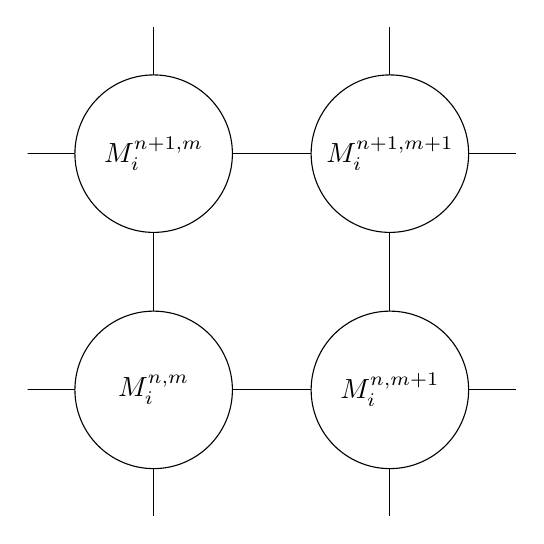
\begin{tikzpicture}
    \clip (-1.6,-1.6) rectangle (4.6,4.6);
    \foreach \X in {-1,0,...,1}
    {\foreach \Y in {-1,0,...,1}
     {\draw[decorate,decoration={aspect=1,amplitude=1mm, segment
    length=5mm}] (\X*3,\Y*3) -- ++(0,3) -- ++(3,0);}}
    \node[circle,draw,inner color=white,minimum size=2cm] at (0,0) {$M_{i}^{n,m}$};
    \node[circle,draw,inner color=white,minimum size=2cm] at (0,3) {$M_{i}^{n+1,m}$};
    \node[circle,draw,inner color=white,minimum size=2cm] at (3,0) {$M_{i}^{n,m+1}$};
    \node[circle,draw,inner color=white,minimum size=2cm] at (3,3) {$M_{i}^{n+1,m+1}$};
  \end{tikzpicture}
\end{center}
 
%%  \begin{tikzpicture}
%%{[start chain,every node/.style={circle,draw},every join/.style=-]
%%\foreach \X in {-2,2,...,-2}
%%{\foreach \Y in {-2,2,...,-2} 
%%  {[start chain]
%%   \node[on chain,join] at (\X+1,\Y+1) {$M_{1}$};
%%   \node[on chain,join] at (\X+1,\Y-1) {$M_{2}$};
%%   \node[on chain,join] at (\X-1,\Y-1) {$M_{3}$};
%%   \node[on chain] at (\X-1,\Y+1) {$M_{4}$};}}}
%%  \end{tikzpicture}

We now extend this analysis to an infinite two-dimensional square lattice. Each
elementary square cell contains four masses $M_i$ for $i\in\left[1, 4\right]$
which are arranged clockwise from the top right. We take $n$ and $m$ to be the
vertical and horizontal directions respectively, so that relative to cell $(n,
m)$ we have cell $(n+1,m)$ above and cell $(n,m+1)$ to the right. With this
setup, we can now label each mass and its displacement uniquely, e.g. $M_i$ in
cell $(n, m)$ is labelled $M_i^{n,m}$ and has displacement $y_i^{n,m}$.

\textit{Note:} Though we use this system to refer to specific masses in
specific cells, the mass of each mass is determined solely by its position in
its cell, i.e. $\forall n,m\in\mathbb{Z}$, the mass of $M_i^{n,m}=M_i$.

Each mass is elastically connected to its direct neighbours, e.g. $M_1^{n,m}$
is connected to $M_2^{n,m}$, $M_4^{n,m}$, $M_2^{n+1,m}$ and $M_4^{n,m+1}$. We
have the spring constant $k$ between masses in the same cell and $\tilde{k}$
between masses in adjacent cells.

Now again we consider only nearest neighbour interactions. Focusing on the
elementary cell $(n,m)$ and its adjacent cells, using Hooke's law and Newton's
2nd law on each of the masses in cell $(n,m)$, we can get a second order
differential equation which is coupled to the displacements of the other masses
it is connected to. For example, considering $M_1^{n,m}$, we get

\begin{align}
  F_1=M_1\frac{d^{2}}{dt^{2}}y_1^{n,m}
      =k\left(y_2^{n,m}+y_4^{n,m}-2y_1^{n,m}\right)+
       \tilde{k}\left(y_2^{n-1,m}+y_4^{n,m+1}-2y_1^{n,m}\right)
\label{eq:2dM1}
\end{align}

Since we can write this differential equation for any of our masses in our
infinite lattice, we would get an infinite number of coupled second order
differential equation. However, similar to the 1d case, using the periodicity
of the lattice and Bloch's theorem once more, we can relate the displacements
of each mass to the corresponding mass in a \textit{base cell} with the lattice
vectors $\kappa_y$ and $\kappa_x$, i.e.

\begin{align}
  y_i^{n+N,m+M}=e^{i\left(N\kappa_y+M\kappa_x\right)}y_i^{n,m}\ \ \ \ 
      \forall N,M\in\mathbb{Z}
\end{align}

With this, instead of an infinite number of equations, we have a set of four
coupled second order differential equations, one for each $y_i^{n,m}$ for
$i\in\left[1,4\right]$. We now drop the superscripts $\left(n,m\right)$ and
assume we have a wave solution of the form  

\begin{align}
  &y_{i}=\hat{y}_{i}e^{-i\Omega t} \\
  \Rightarrow &\frac{d^{2}}{dt^{2}}y_{i}=-\Omega^{2}y_{i} \\
  \Rightarrow &F_{i}=-M_i\Omega_i^{2}y_{i} \label{eq:N2L}
\end{align}

where $\Omega$ is the frequency of the wave and $\hat{y}_{n}$ is the complex
amplitude. We can now rewrite \eqref{eq:2dM1} as

\begin{align}
  M_1\Omega_1^{2}y_1
      &=k\left(2y_1-y_2-y_4\right)+
       \tilde{k}\left(2y_1-y_{2}e^{-i\kappa_y}-y_{4}e^{i\kappa_x}\right) \\
      &=\left(2k+2\tilde{k}\right)y_1+\left(-k-\tilde{k}e^{-i\kappa_y}\right)y_2+
       \left(-k-\tilde{k}e^{i\kappa_x}\right)y_4
\end{align}

By constructing this equation for each $y_i$, we can reformulated these four
difference equations as an eigenvalue problem

\begin{align}
  \left[\matr{A(\kappa)}+\matr{\Omega}\matr{M}\right]\vec{y}=\vec{0}
\end{align}

where $\matr{\Omega}=\diag\left(\left\{\Omega_i^2\right\}\right)$,
$\matr{M}=\diag\left(\left\{M_i^2\right\}\right)$,
$\vec{y}=\left[\left\{y_i\right\}\right]^T$ and

\begin{align}
  \matr{A(\kappa)}=\left[
\begin{array}{cccc}
2k+\tilde{k} & -k-\tilde{k}e^{-i\kappa_{y}} & 0 & -k-\tilde{k}e^{i\kappa_{x}}\\
-k-\tilde{k}e^{i\kappa_{y}} & 2k+\tilde{\tilde{k}} & -k-\tilde{k}e^{i\kappa_{x}} & 0\\
0 & -k-\tilde{k}e^{-i\kappa_{x}} & 2k+\tilde{\tilde{k}} & -k-\tilde{k}e^{i\kappa_{y}}\\
-k-\tilde{k}e^{-i\kappa_{x}} & 0 & -k-\tilde{k}e^{-i\kappa_{y}} & 2k+\tilde{\tilde{k}}
\end{array}\right]
\end{align}

Therefore, we can solve for the eigenvalues and eigenvectors of this equation.
The eigenvalues of this equation correspond to the frequency of waves,
$\Omega$, which are allowed through our lattice while the eigenvectors
correspond to the displacement of the masses, $y_i$. However, the next question
arises: How should we vary $\kappa$ so that we get a good enough picture of the
full dispersion relation of our 2d lattice?

To answer this question, we first have to discuss the theory of Brillouin zones.
%TODO: Complete discussion of square lattice

\subsection{Brillouin zones}
\label{brizones}
The concept of Brillouin zones was first defined by Leon Brillouin in his book
on wave propagation in periodic structures.\cite{brillouin}
%TODO: Complete discussion of brillouin zones

\section{2d hexagonal lattice}
We will now consider how waves propagate across a 2d lattice made of hexagonal elementary cells. 

%TODO: Add image to show model
Consider an infinite 2d plane made of hexagonal unit cells of six masses $M_i$
for $i\in\left[1,6\right]$, which are arranged in an inner hexagon rotated
$\frac{\pi}{6}$ relative to each cell. Now we take the spring constant to be $k$
between masses within the same cell and $\tilde{k}$ between masses in adjacent
cells.
%TODO: Complete discussion of hexagonal lattice


\chapter{Perturbed system}
\label{perturbed}

\section{Band gap formed}

\section{2d hexagonal strip}

\section{Formulation of semi-infinite hexagonal lattice}

\chapter{Scattering simulation}
\label{scattering}

\section{Simulation results}

\chapter{Complex bends}
\label{complexbends}
Now that we have built up the foundation of how we can force a wave to
propagate in a specific direction in a topologically repeating material or
metamaterial, we want to see just how robust this phenomenon is based on the
shape of the boundary, i.e. just how much can we bend the wave?

\textit{Note:} For the hexagonal simulations, we will specifically be using the
same top and bottom cells as Figure~\ref{fig:hexstdrotstraight}, which is with
alternating masses as defined in Figure~\ref{fig:hexstripMrotated}. And for the
kagome simulations, we will specifically be using the same top and bottom cells
as Figure~\ref{fig:kagomestd}.

\section{Gentle and sharp straight bends}
So far we have seen just straight line boundaries, but can this work for bent
boundaries too? Due to the way we set up our lattice (with the strips getting
higher as we go from left to right), there are two kinds of bends we can make
straight away. The 'gentle' bend where we bend the boundary upwards, and the
'sharp' bend where we bend the boundary downwards.

\begin{figure}[!h]
\centering
\begin{subfigure}[b]{.5\textwidth}
  \centering
  \includegraphics[width=0.8\linewidth]{imgs/gentlebendarr.png}
  \caption{Arrangement of cells to form a gentle bend.}
  \label{fig:sub1}
\end{subfigure}%
\begin{subfigure}[b]{.5\textwidth}
  \centering
  \includegraphics[width=1\linewidth]{imgs/gentlebendscat.png}
  \caption{The plot of $|y_i|$ for each mass in each cell.}
  \label{fig:sub2}
\end{subfigure}

\medskip
\centering
\begin{subfigure}[b]{.5\textwidth}
  \centering
  \includegraphics[width=0.8\linewidth]{imgs/kagomegentlebendarr.png}
  \caption{Arrangement of cells to form a gentle bend.}
  \label{fig:sub1}
\end{subfigure}%
\begin{subfigure}[b]{.5\textwidth}
  \centering
  \includegraphics[width=1\linewidth]{imgs/kagomegentlebendscat.png}
  \caption{The plot of $|y_i|$ for each mass in each cell.}
  \label{fig:kagomegentlebendscat}
\end{subfigure}
\caption{Simulation of scattering hexagonal and kagome finite lattices with a
  gentle bend.}
\label{fig:gentlebend}
\end{figure}

\begin{figure}[!h]
\centering
\begin{subfigure}[b]{.5\textwidth}
  \centering
  \includegraphics[width=0.8\linewidth]{imgs/sharpbendarr.png}
  \caption{Arrangement of cells to form a sharp bend.}
  \label{fig:sub1}
\end{subfigure}%
\begin{subfigure}[b]{.5\textwidth}
  \centering
  \includegraphics[width=1\linewidth]{imgs/sharpbendscat.png}
  \caption{The plot of $|y_i|$ for each mass in each cell.}
  \label{fig:sub2}
\end{subfigure}

\medskip
\centering
\begin{subfigure}[b]{.5\textwidth}
  \centering
  \includegraphics[width=0.8\linewidth]{imgs/kagomesharpbendarr.png}
  \caption{Arrangement of cells to form a sharp bend.}
  \label{fig:sub1}
\end{subfigure}%
\begin{subfigure}[b]{.5\textwidth}
  \centering
  \includegraphics[width=1\linewidth]{imgs/kagomesharpbendscat.png}
  \caption{The plot of $|y_i|$ for each mass in each cell.}
  \label{fig:sub2}
\end{subfigure}
\caption{Simulation of scattering on the hexagonal and kagome finite lattice
  with a sharp bend.}
\label{fig:sharpbend}
\end{figure}

Amazingly, our systems are able to stand up to both of these bends as we can see
in Figure~\ref{fig:gentlebend} and Figure~\ref{fig:sharpbend}, and these type
of bends may be useful in the production of lenses.\cite{negrefraclens}

\section{Curved bends}
So it can travel around gentle and sharp straight bends; it is only natural to
then wonder if it can propagate as well along a curved bend. Being able to bend
energy around a corner could be useful in the creation of an invisibility
cloak.\cite{emcloak}

\begin{figure}[!h]
\centering
\begin{subfigure}[b]{.5\textwidth}
  \centering
  \includegraphics[width=0.8\linewidth]{imgs/curvedbendarr.png}
  \caption{Arrangement of cells to form a curved bend.}
  \label{fig:sub1}
\end{subfigure}%
\begin{subfigure}[b]{.5\textwidth}
  \centering
  \includegraphics[width=1\linewidth]{imgs/curvedbendscat.png}
  \caption{The plot of $|y_i|$ for each mass in each cell.}
  \label{fig:sub2}
\end{subfigure}

\medskip
\centering
\begin{subfigure}[b]{.5\textwidth}
  \centering
  \includegraphics[width=0.8\linewidth]{imgs/kagomecurvedbendarr.png}
  \caption{Arrangement of cells to form a curved bend.}
  \label{fig:sub1}
\end{subfigure}%
\begin{subfigure}[b]{.5\textwidth}
  \centering
  \includegraphics[width=1\linewidth]{imgs/kagomecurvedbendscat.png}
  \caption{The plot of $|y_i|$ for each mass in each cell.}
  \label{fig:sub2}
\end{subfigure}
\caption{Simulation of scattering on the hexagonal and kagome finite lattice
  with curved bend.}
\label{fig:curvedbend}
\end{figure}

\section{Energy splitting and merging}
One of the applications of metamaterials that we have discussed is splitting
and also focusing energy.\cite{toposplit,diremi,antennasol} And we see that we
are able to get the energy splitting behaviour in Figure~\ref{fig:esplit}.
Unfortunately we are unable to model the energy merging scenario in our system
as we do not model the flow of energy over time, but just the overall steady
state wave. However, we can imagine that we could have sources of excitation at
the three branches and have them converge onto the single branch.

\begin{figure}[!h]
\centering
\begin{subfigure}[b]{.5\textwidth}
  \centering
  \includegraphics[width=0.8\linewidth]{imgs/esplitarr.png}
  \caption{Arrangement of cells to form a 3-way split.}
  \label{fig:sub1}
\end{subfigure}%
\begin{subfigure}[b]{.5\textwidth}
  \centering
  \includegraphics[width=1\linewidth]{imgs/esplitscat.png}
  \caption{The plot of $|y_i|$ for each mass in each cell.}
  \label{fig:sub2}
\end{subfigure}

\medskip
\centering
\begin{subfigure}[b]{.5\textwidth}
  \centering
  \includegraphics[width=0.8\linewidth]{imgs/kagomeesplitarr.png}
  \caption{Arrangement of cells to form a 3-way split.}
  \label{fig:sub1}
\end{subfigure}%
\begin{subfigure}[b]{.5\textwidth}
  \centering
  \includegraphics[width=1\linewidth]{imgs/kagomeesplitscat.png}
  \caption{The plot of $|y_i|$ for each mass in each cell.}
  \label{fig:sub2}
\end{subfigure}
\caption{Simulation of scattering on the hexagonal and kagome finite lattice
  with a 3-way split, modelling a 3-way energy splitter.}
\label{fig:esplit}
\end{figure}


\chapter{Evaluation}
% TODO: Compare results to those of more complex models; look at other papers
% and use their parameters

\section{Further work}
% TODO: Can split into what we can do in terms of different perturbations/
% grading etc; but also look at computing side, e.g. split into classes so
% easier to run simulations and get dispersion curves etc
% - evaluate the robustness of our systems (real life production isn't
% perfect), how resistant it is to small imperfections

\chapter{Conclusion}
Herein we have constructed various different model mass-spring lattices on
which we have built up not just the mathematics, but also the codes, to allow
us to analyse the effects of a topological perturbation. This has led us to
discovering various different configurations of lattices which permit a wide
range of wave propagation manipulation. As we see that our results match those
obtained from other models, we anticipate that our model system is a good
approximation and can be used to model more complex waves.
%TODO: Complete


\bibliographystyle{unsrt}
\bibliography{bibs/bibliography}

\end{document}
